\documentclass[tikz,border=2pt]{standalone}
\usepackage{amsmath}\usepackage{pgfplots}\usepgfplotslibrary{groupplots}\pgfplotsset{compat=1.18}
\definecolor{cA}{HTML}{2166AC}\definecolor{cB}{HTML}{1B9E77}\definecolor{cC}{HTML}{D95F02}\definecolor{cD}{HTML}{C51B7D}\definecolor{cE}{HTML}{7570B3}
\begin{document}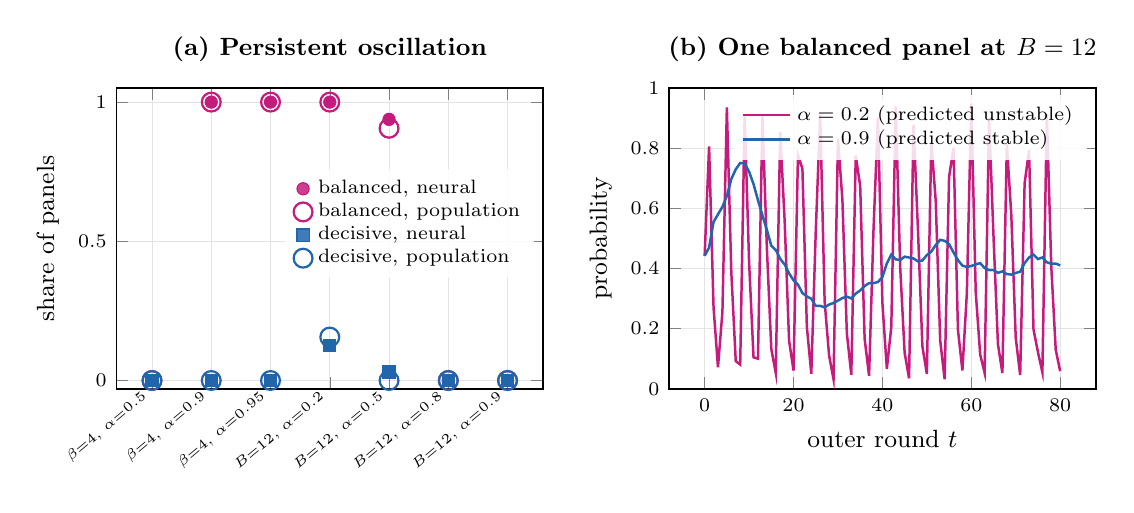
\begin{tikzpicture}
\begin{groupplot}[group style={group size=2 by 1, horizontal sep=1.6cm}, width=7.0cm, height=5.4cm, tick label style={font=\scriptsize}, label style={font=\small}, title style={font=\small\bfseries}, grid=major, grid style={draw=gray!22, line width=0.25pt}, axis line style={black, line width=0.6pt}, legend style={font=\scriptsize, draw=none, fill=white, fill opacity=0.85, text opacity=1, cells={anchor=west}, row sep=-2pt}]
\nextgroupplot[title={(a) Persistent oscillation}, ylabel={share of panels}, ymin=-0.03, ymax=1.05, xtick={0,1,2,3,4,5,6}, xticklabels={{$\beta{=}4$, $\alpha{=}0.5$},{$\beta{=}4$, $\alpha{=}0.9$},{$\beta{=}4$, $\alpha{=}0.95$},{$B{=}12$, $\alpha{=}0.2$},{$B{=}12$, $\alpha{=}0.5$},{$B{=}12$, $\alpha{=}0.8$},{$B{=}12$, $\alpha{=}0.9$}}, x tick label style={rotate=40, anchor=east, font=\tiny}, legend style={at={(0.98,0.55)}, anchor=east}]
\addplot[only marks, cD, mark=*, mark size=2.2pt] coordinates {(0,0.000) (1,1.000) (2,1.000) (3,1.000) (4,0.938) (5,0.000) (6,0.000)}; \addlegendentry{balanced, neural}
\addplot[only marks, cD, mark=o, mark size=3.4pt, thick] coordinates {(0,0.000) (1,1.000) (2,1.000) (3,1.000) (4,0.906) (5,0.000) (6,0.000)}; \addlegendentry{balanced, population}
\addplot[only marks, cA, mark=square*, mark size=2.2pt] coordinates {(0,0.000) (1,0.000) (2,0.000) (3,0.125) (4,0.031) (5,0.000) (6,0.000)}; \addlegendentry{decisive, neural}
\addplot[only marks, cA, mark=o, mark size=3.4pt, thick] coordinates {(0,0.000) (1,0.000) (2,0.000) (3,0.156) (4,0.000) (5,0.000) (6,0.000)}; \addlegendentry{decisive, population}
\nextgroupplot[title={(b) One balanced panel at $B=12$}, xlabel={outer round $t$}, ylabel={probability}, ymin=0, ymax=1, legend style={at={(0.98,0.98)}, anchor=north east}]
\addplot[cD, line width=0.9pt] coordinates {(0,0.44241) (1,0.80631) (2,0.27234) (3,0.071667) (4,0.2556) (5,0.9358) (6,0.38794) (7,0.092314) (8,0.080731) (9,0.91138) (10,0.4214) (11,0.10476) (12,0.10033) (13,0.90648) (14,0.46905) (15,0.13215) (16,0.053187) (17,0.85421) (18,0.55951) (19,0.16011) (20,0.060731) (21,0.7768) (22,0.7327) (23,0.20624) (24,0.050293) (25,0.52196) (26,0.91308) (27,0.29109) (28,0.11117) (29,0.03195) (30,0.83198) (31,0.62867) (32,0.18493) (33,0.046756) (34,0.77583) (35,0.67487) (36,0.16643) (37,0.043403) (38,0.53025) (39,0.90205) (40,0.28507) (41,0.06634) (42,0.20563) (43,0.93916) (44,0.40474) (45,0.12058) (46,0.034923) (47,0.87785) (48,0.52899) (49,0.14099) (50,0.049594) (51,0.8225) (52,0.62481) (53,0.16139) (54,0.031946) (55,0.70436) (56,0.80152) (57,0.19612) (58,0.06097) (59,0.31782) (60,0.94909) (61,0.322) (62,0.11422) (63,0.053159) (64,0.90097) (65,0.50732) (66,0.1484) (67,0.052455) (68,0.81304) (69,0.57973) (70,0.16994) (71,0.045778) (72,0.68329) (73,0.79367) (74,0.19788) (75,0.12205) (76,0.054949) (77,0.91416) (78,0.40641) (79,0.13054) (80,0.058688)}; \addlegendentry{$\alpha=0.2$ (predicted unstable)}
\addplot[cA, line width=0.9pt] coordinates {(0,0.44241) (1,0.46995) (2,0.55469) (3,0.58051) (4,0.60556) (5,0.64115) (6,0.69787) (7,0.73016) (8,0.7512) (9,0.74975) (10,0.72225) (11,0.68098) (12,0.62714) (13,0.5771) (14,0.52888) (15,0.4759) (16,0.46189) (17,0.43241) (18,0.4137) (19,0.38392) (20,0.36109) (21,0.34666) (22,0.31855) (23,0.30752) (24,0.29961) (25,0.27585) (26,0.27626) (27,0.27088) (28,0.2804) (29,0.28554) (30,0.29345) (31,0.30216) (32,0.30682) (33,0.30076) (34,0.31678) (35,0.32739) (36,0.34178) (37,0.35172) (38,0.35154) (39,0.35546) (40,0.37197) (41,0.41722) (42,0.44631) (43,0.43068) (44,0.42849) (45,0.43963) (46,0.43673) (47,0.43365) (48,0.42411) (49,0.42679) (50,0.44494) (51,0.45642) (52,0.47837) (53,0.4958) (54,0.49218) (55,0.48156) (56,0.4536) (57,0.42818) (58,0.40991) (59,0.40535) (60,0.40849) (61,0.41403) (62,0.41809) (63,0.40173) (64,0.39525) (65,0.39528) (66,0.38589) (67,0.39064) (68,0.38174) (69,0.3801) (70,0.38538) (71,0.38983) (72,0.41816) (73,0.43702) (74,0.44649) (75,0.43171) (76,0.43701) (77,0.42118) (78,0.41599) (79,0.4168) (80,0.41056)}; \addlegendentry{$\alpha=0.9$ (predicted stable)}
\end{groupplot}
\end{tikzpicture}\end{document}
